\documentclass[9pt]{IEEEtran}

\usepackage[english]{babel}
\usepackage{graphicx}
\usepackage{epstopdf}
\usepackage{fancyhdr}
\usepackage{amsmath}
\usepackage{amsthm}
\usepackage{amssymb}
\usepackage{url}
\usepackage{array}
\usepackage{textcomp}
\usepackage{listings}
\usepackage{hyperref}
\usepackage{xcolor}
\usepackage{colortbl}
\usepackage{float}
\usepackage{gensymb}
\usepackage{longtable}
\usepackage{supertabular}
\usepackage{multicol}

\usepackage[utf8]{inputenc}

\usepackage[T1]{fontenc}
\usepackage{lmodern}
\input{glyphtounicode}
\pdfgentounicode=1

\graphicspath{{./figures/}{./report_temp_figs/}{./}}
\DeclareGraphicsExtensions{.pdf,.png,.jpg,.eps}

% correct bad hyphenation here
\hyphenation{op-tical net-works semi-conduc-tor trig-gs}

% ============================================================================================

\title{\vspace{0ex}
Exercise 1: Optical Flow (Lucas-Kanade and Horn-Schunck)}

\author{Dino D\v{z}aferagi\'c\vspace{-4.0ex}}

% ============================================================================================

\begin{document}

\maketitle

\section{Introduction}
In this exercise, I implemented dense optical flow with two methods: Lucas-Kanade (LK) and Horn-Schunck (HS).  
I used grayscale images and normalized values to $[0,1]$. I computed image gradients with Gaussian derivatives.  
LK uses local least-squares in a window. HS uses an iterative update with a smoothness term controlled by $\lambda$.

\section{Experiments}
\subsection{Required synthetic sanity check}
Figure~\ref{fig:synthetic_inputs} and Figure~\ref{fig:synthetic_flow} show the rotated random-noise test.  
Both methods recover the expected rotation pattern. HS gives a smoother dense field. LK gives a less smooth field because it solves the flow only from local windows.

\begin{figure}[H]
    \centering
    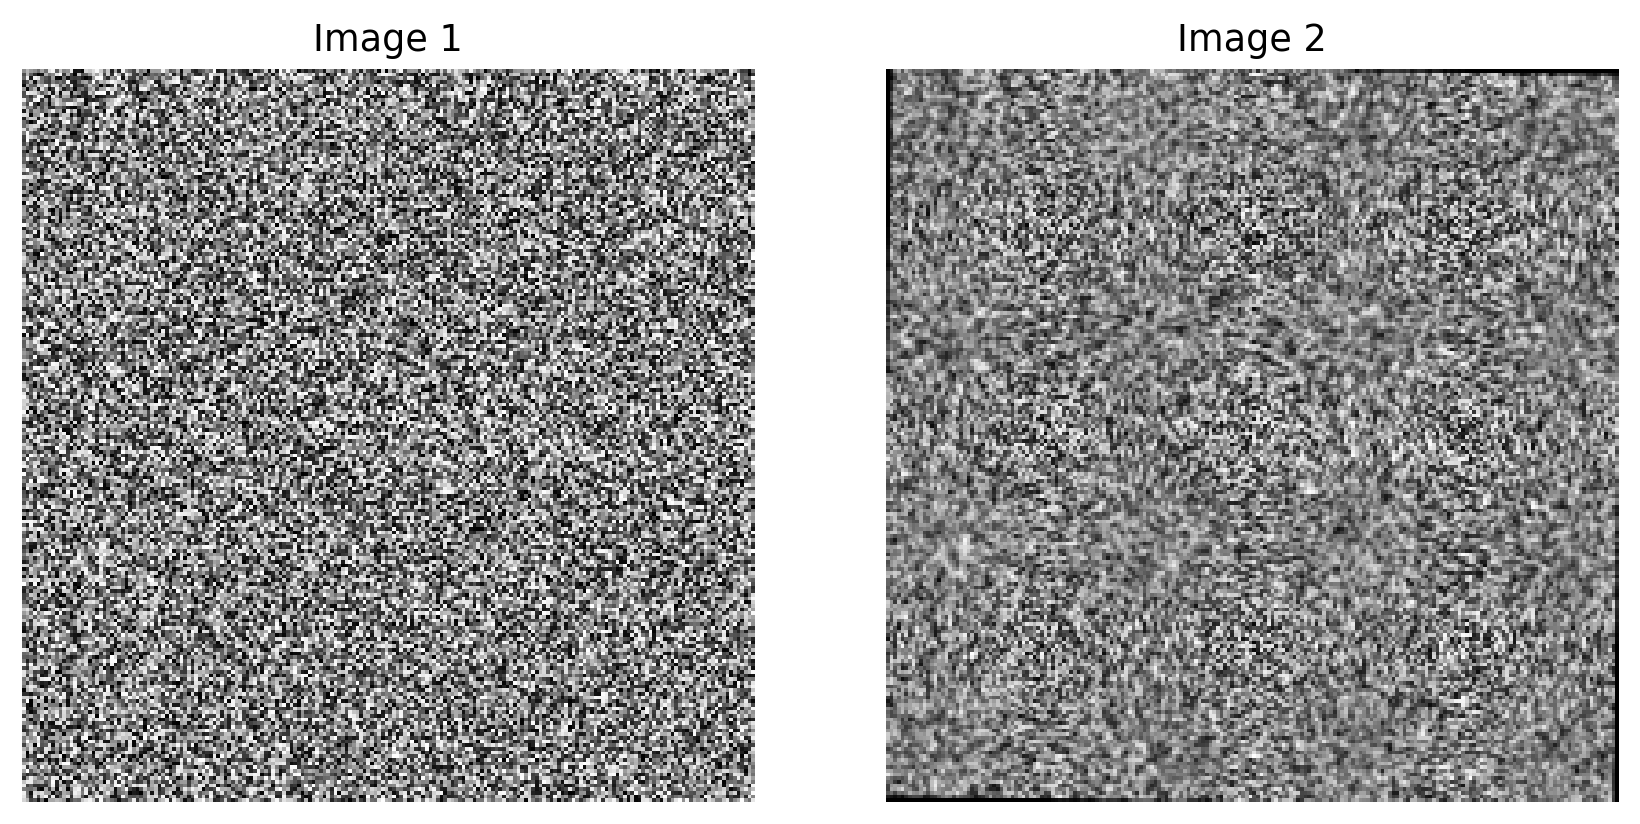
\includegraphics[width=1\columnwidth]{figure1_inputs.png}
    \caption{Synthetic rotated random-noise pair (input images).}
    \label{fig:synthetic_inputs}
\end{figure}

\begin{figure}[H]
    \centering
    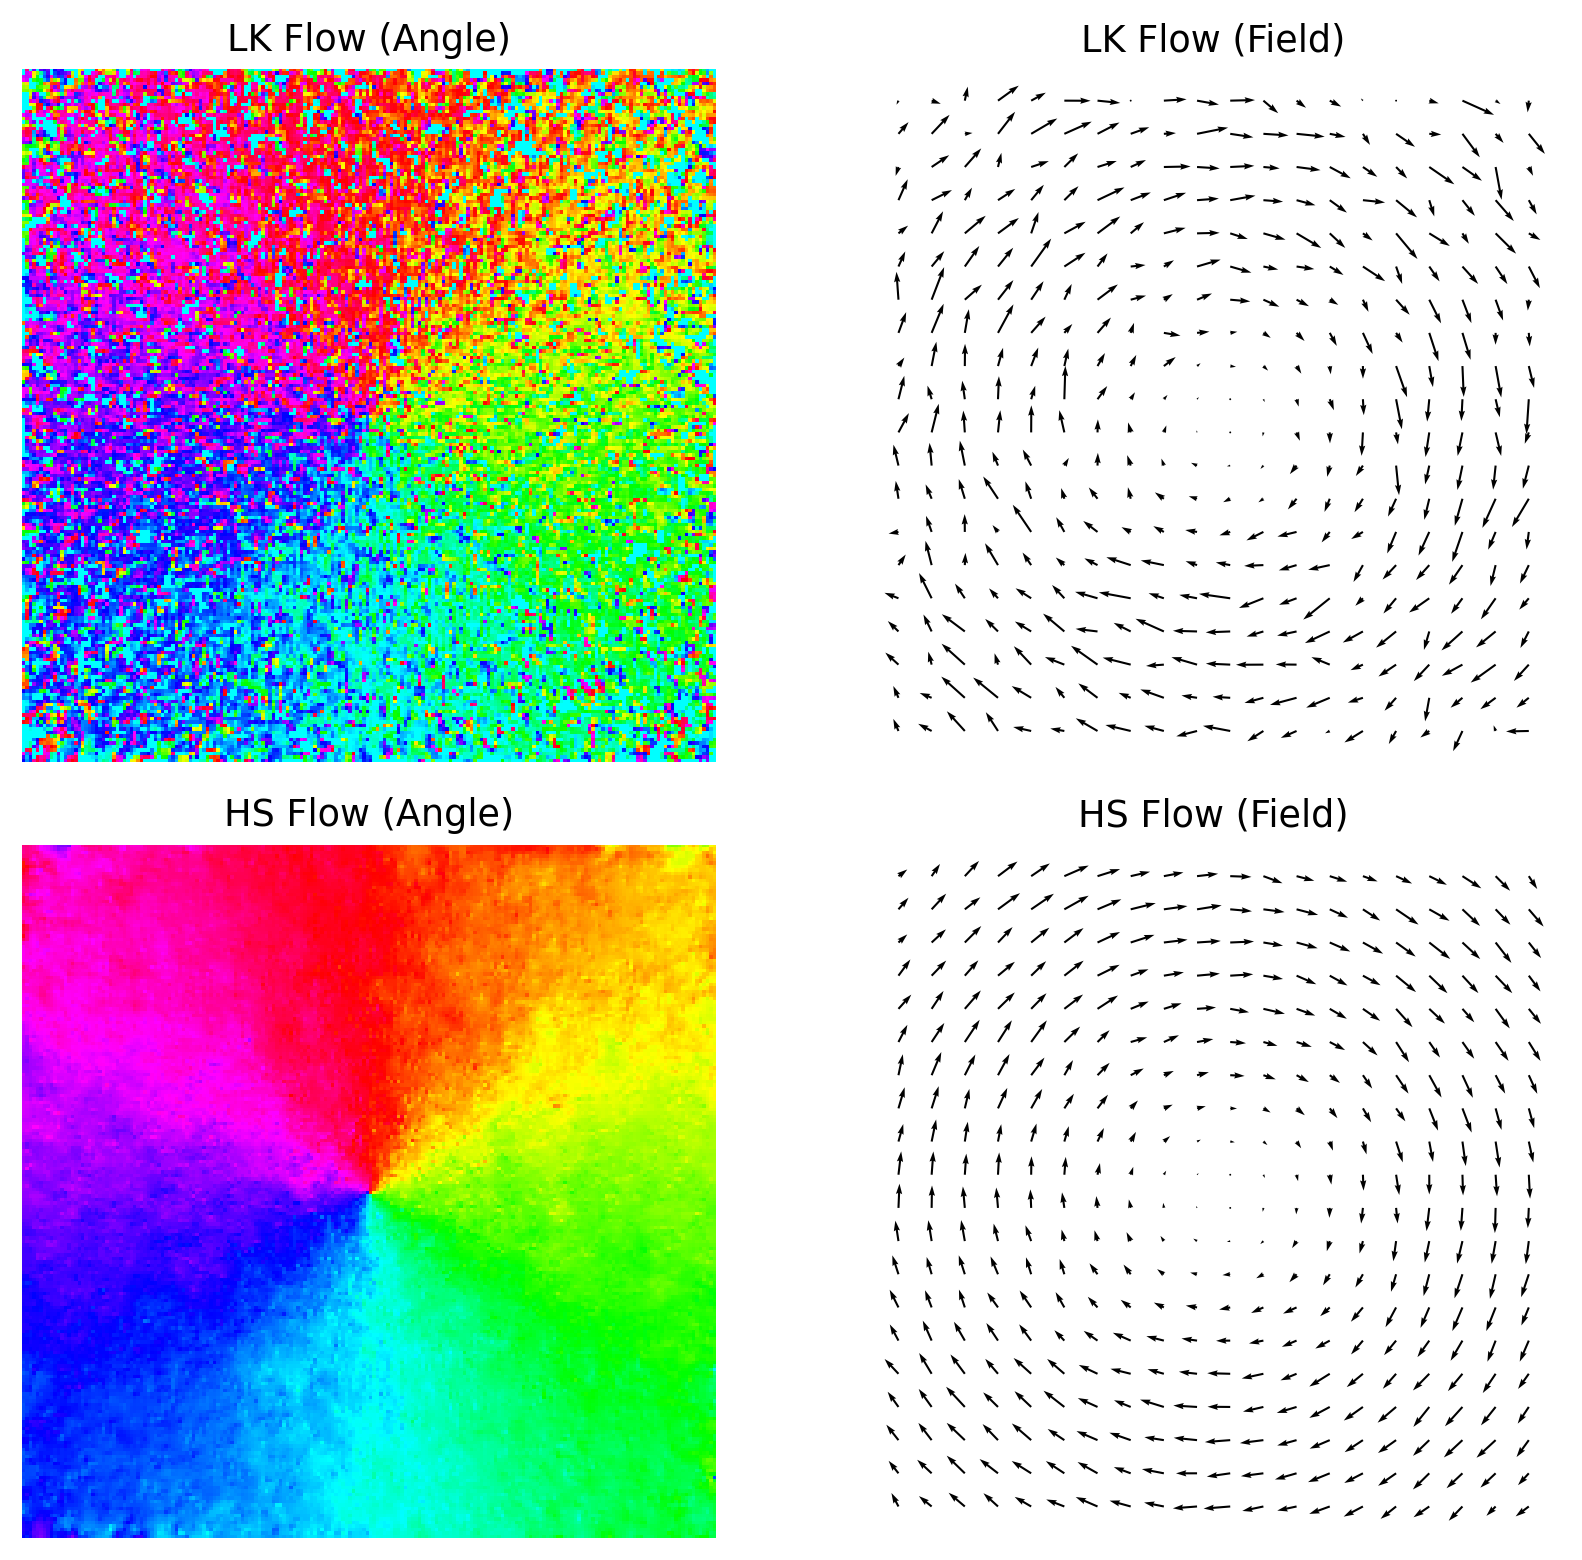
\includegraphics[width=1\columnwidth]{figure1_flows.png}
    \caption{Synthetic test: LK (top row) and HS (bottom row).}
    \label{fig:synthetic_flow}
\end{figure}

\subsection{Real-image pair example (disparity cporta)}
Figure~\ref{fig:cporta_inputs} and Figure~\ref{fig:cporta_flow} show results on the real \texttt{cporta} pair.  
HS again gives a dense flow map. LK is sparse in low-texture areas and shows local outliers. This is a common LK failure case.

\begin{figure}[H]
    \centering
    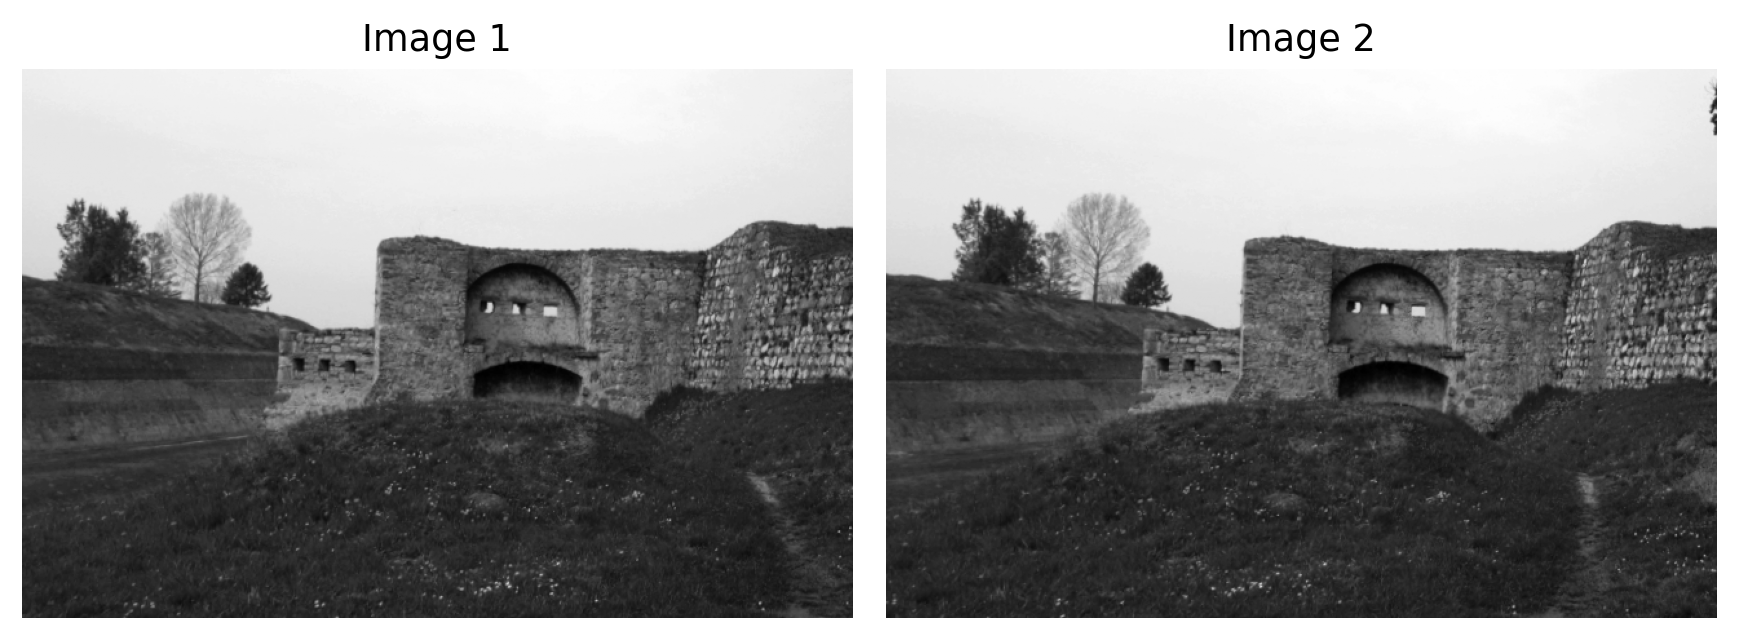
\includegraphics[width=1\columnwidth]{figure4_inputs.png}
    \caption{Disparity cporta pair (input images).}
    \label{fig:cporta_inputs}
\end{figure}

\begin{figure}[H]
    \centering
    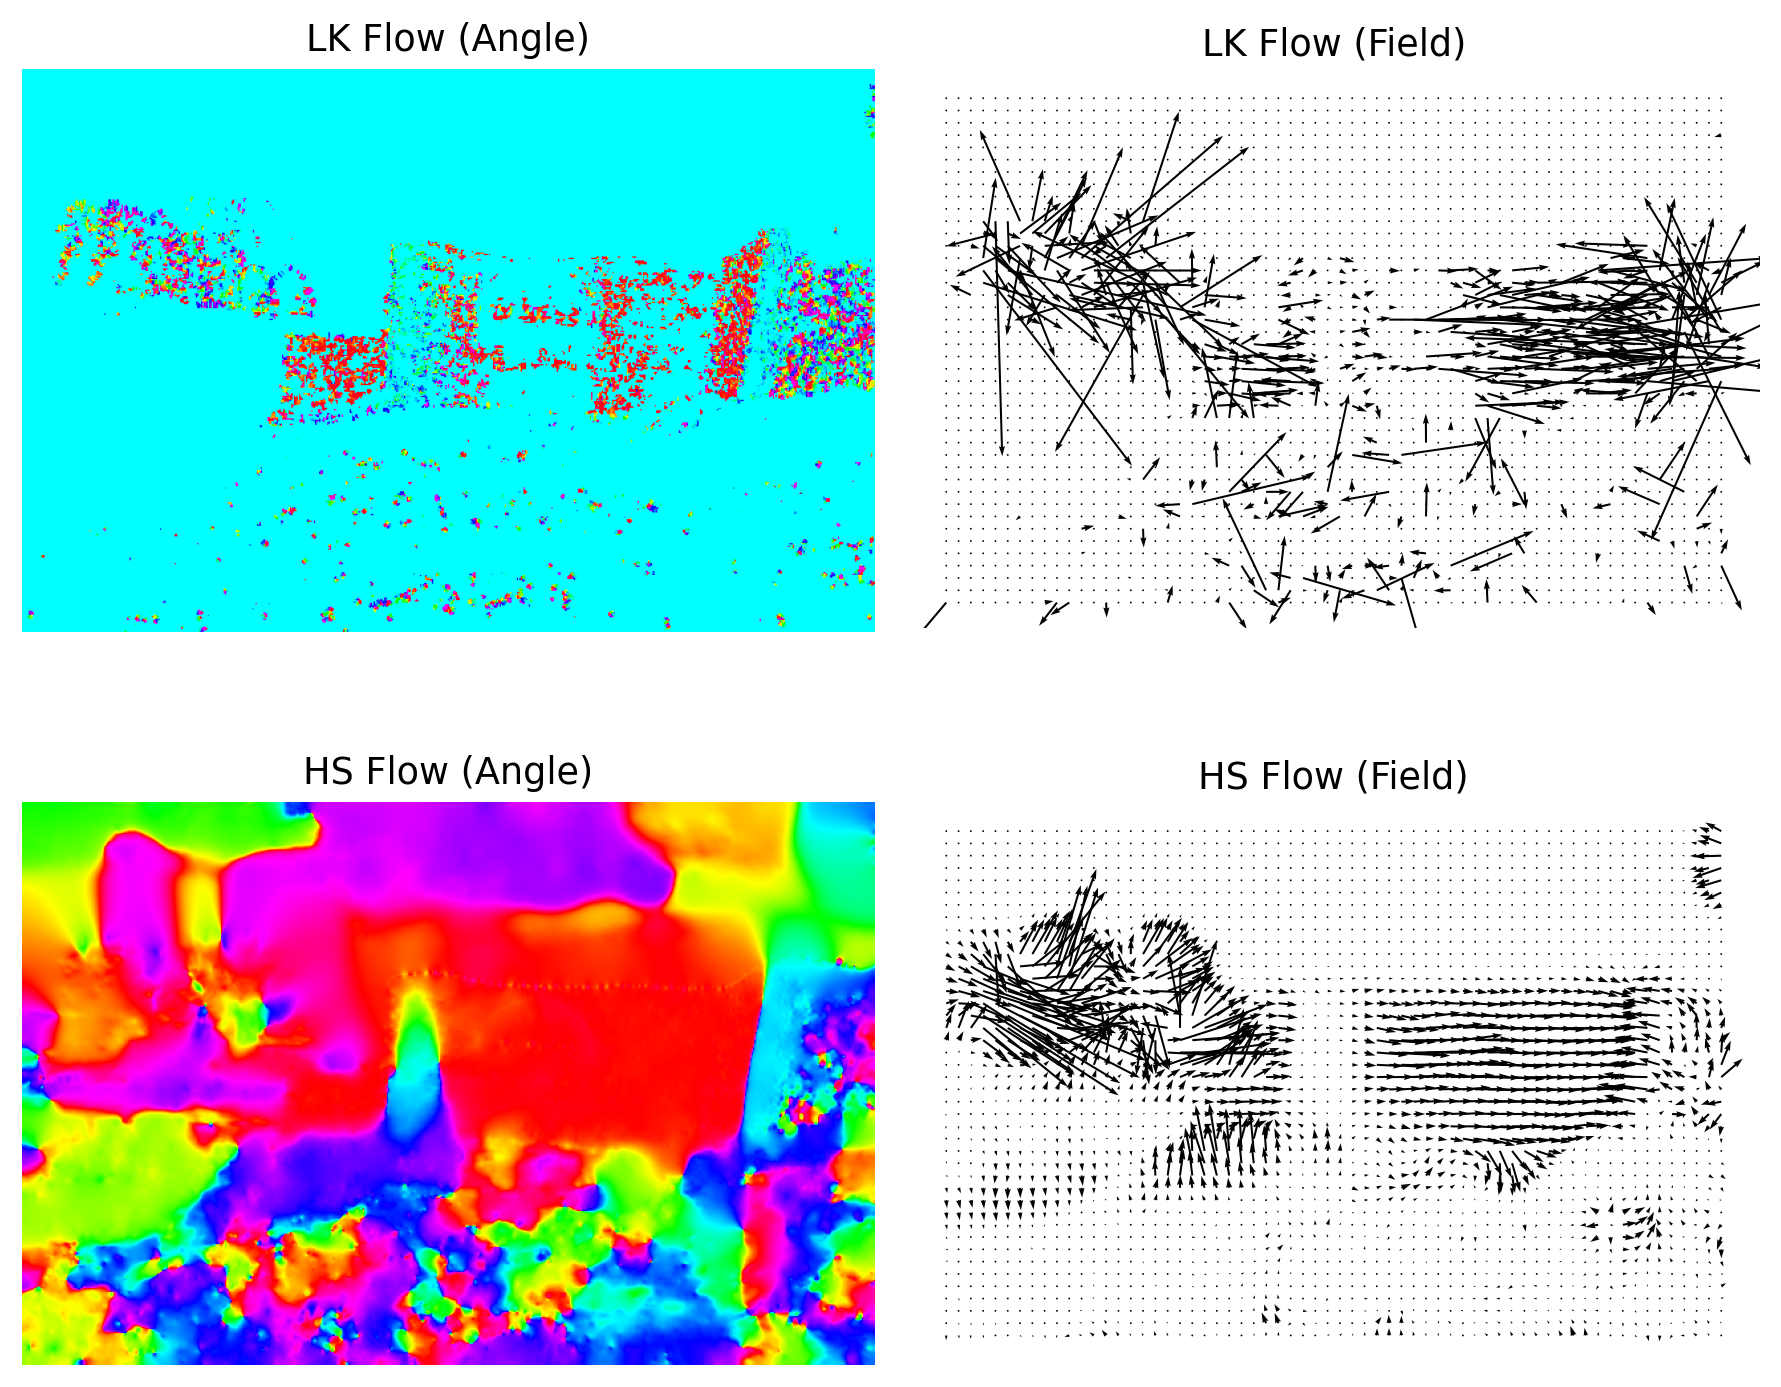
\includegraphics[width=1\columnwidth]{figure4_flows.png}
    \caption{Disparity cporta: LK (top row) and HS (bottom row).}
    \label{fig:cporta_flow}
\end{figure}

\subsection{Parameter impact and speed}
For LK, the best residual is at $N=5$ (\(1.1170\times10^{-2}\)).  
For HS, lower \(\lambda\) gives lower residual in this setup. The best value is \(\lambda=0.1\) with \(1000\) iterations (\(8.2025\times10^{-3}\)).  
More HS iterations improve residual, but they also increase runtime.

\begin{table}[h]
    \centering
    \caption{Runtime and optimization summary}
    \begin{tabular}{|l|c|c|}
        \hline
        Method/setup & Residual & Time \\
        \hline
        LK (\(N=5\)) & \(1.1170\times10^{-2}\) & 18.56 ms \\
        HS (\(\lambda=0.5\), 1000 iters) & \(1.0373\times10^{-2}\) & 817.55 ms \\
        HS zero init (1000 iters) & \(1.0373\times10^{-2}\) & 1311.84 ms \\
        LK init + HS (300 iters) & \(1.0492\times10^{-2}\) & 291.77 ms \\
        \hline
    \end{tabular}
    \label{tab:runtime}
\end{table}

Initializing HS with LK reduced total time by about \(4.5\times\) relative to the measured HS zero-init run, with only a small residual increase (\(\approx 1.2\times10^{-4}\)).
This gives a good speed/accuracy tradeoff.

\subsection{Additional part: pyramidal LK}
I also implemented iterative LK on one scale and pyramidal LK.  
On a large-translation synthetic pair, plain LK gave residual \(1.55\times10^{-1}\), iterative LK \(2.70\times10^{-1}\), and pyramidal LK \(8.22\).  
This result shows that my current pyramid settings are not tuned yet.  
The likely cause is scale-to-scale error build-up and poor parameter settings between levels.

\begin{figure}[H]
    \centering
    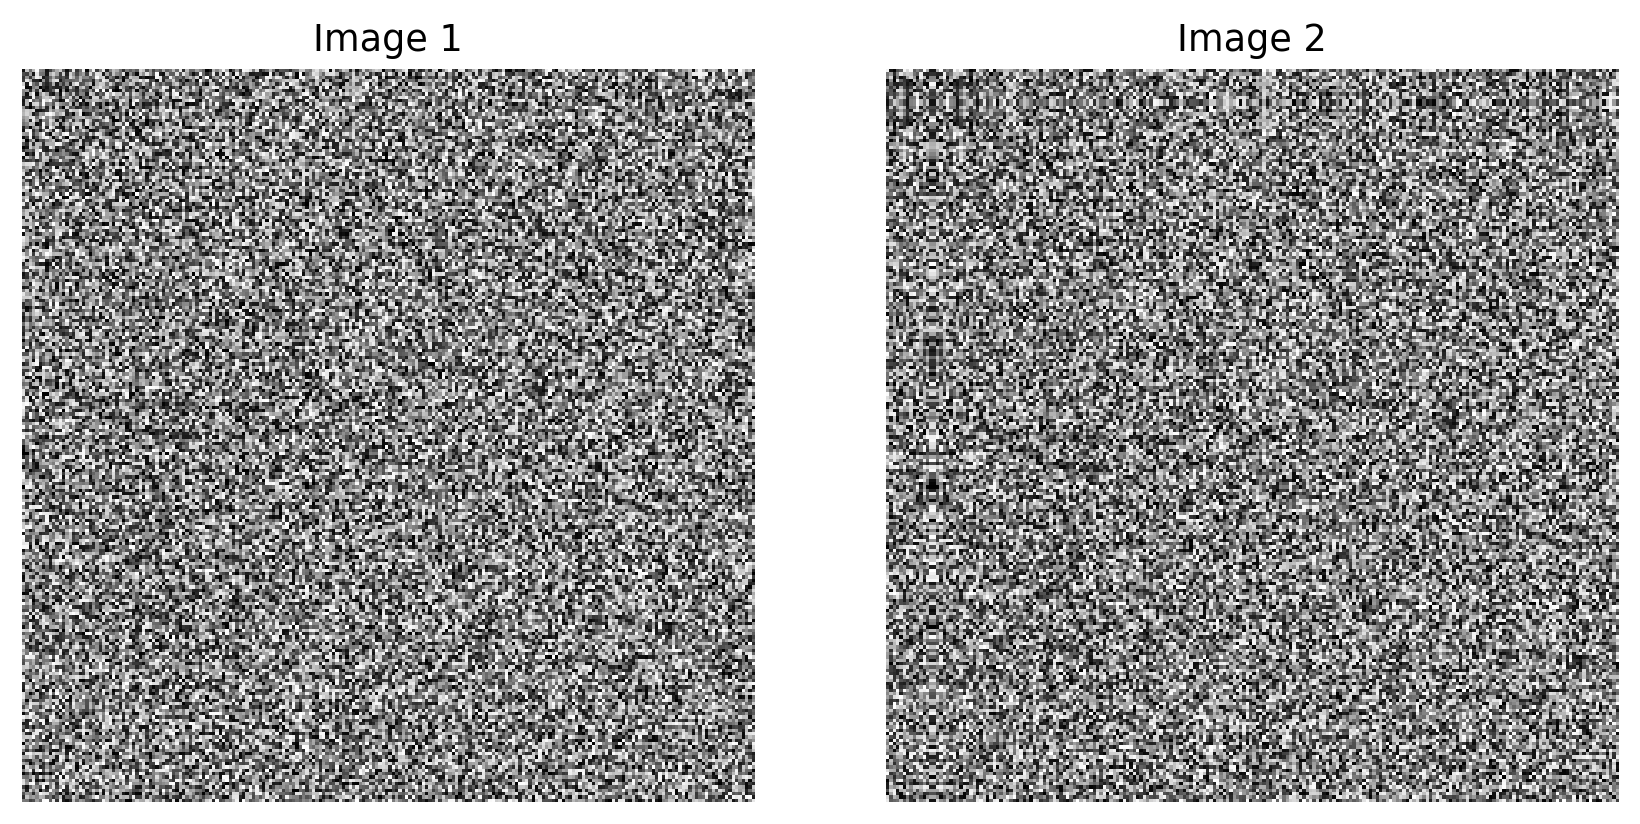
\includegraphics[width=1\columnwidth]{figure_pyr_inputs.png}
    \caption{Large-motion synthetic pair used for the pyramidal LK test.}
    \label{fig:pyr_inputs}
\end{figure}

\begin{figure}[H]
    \centering
    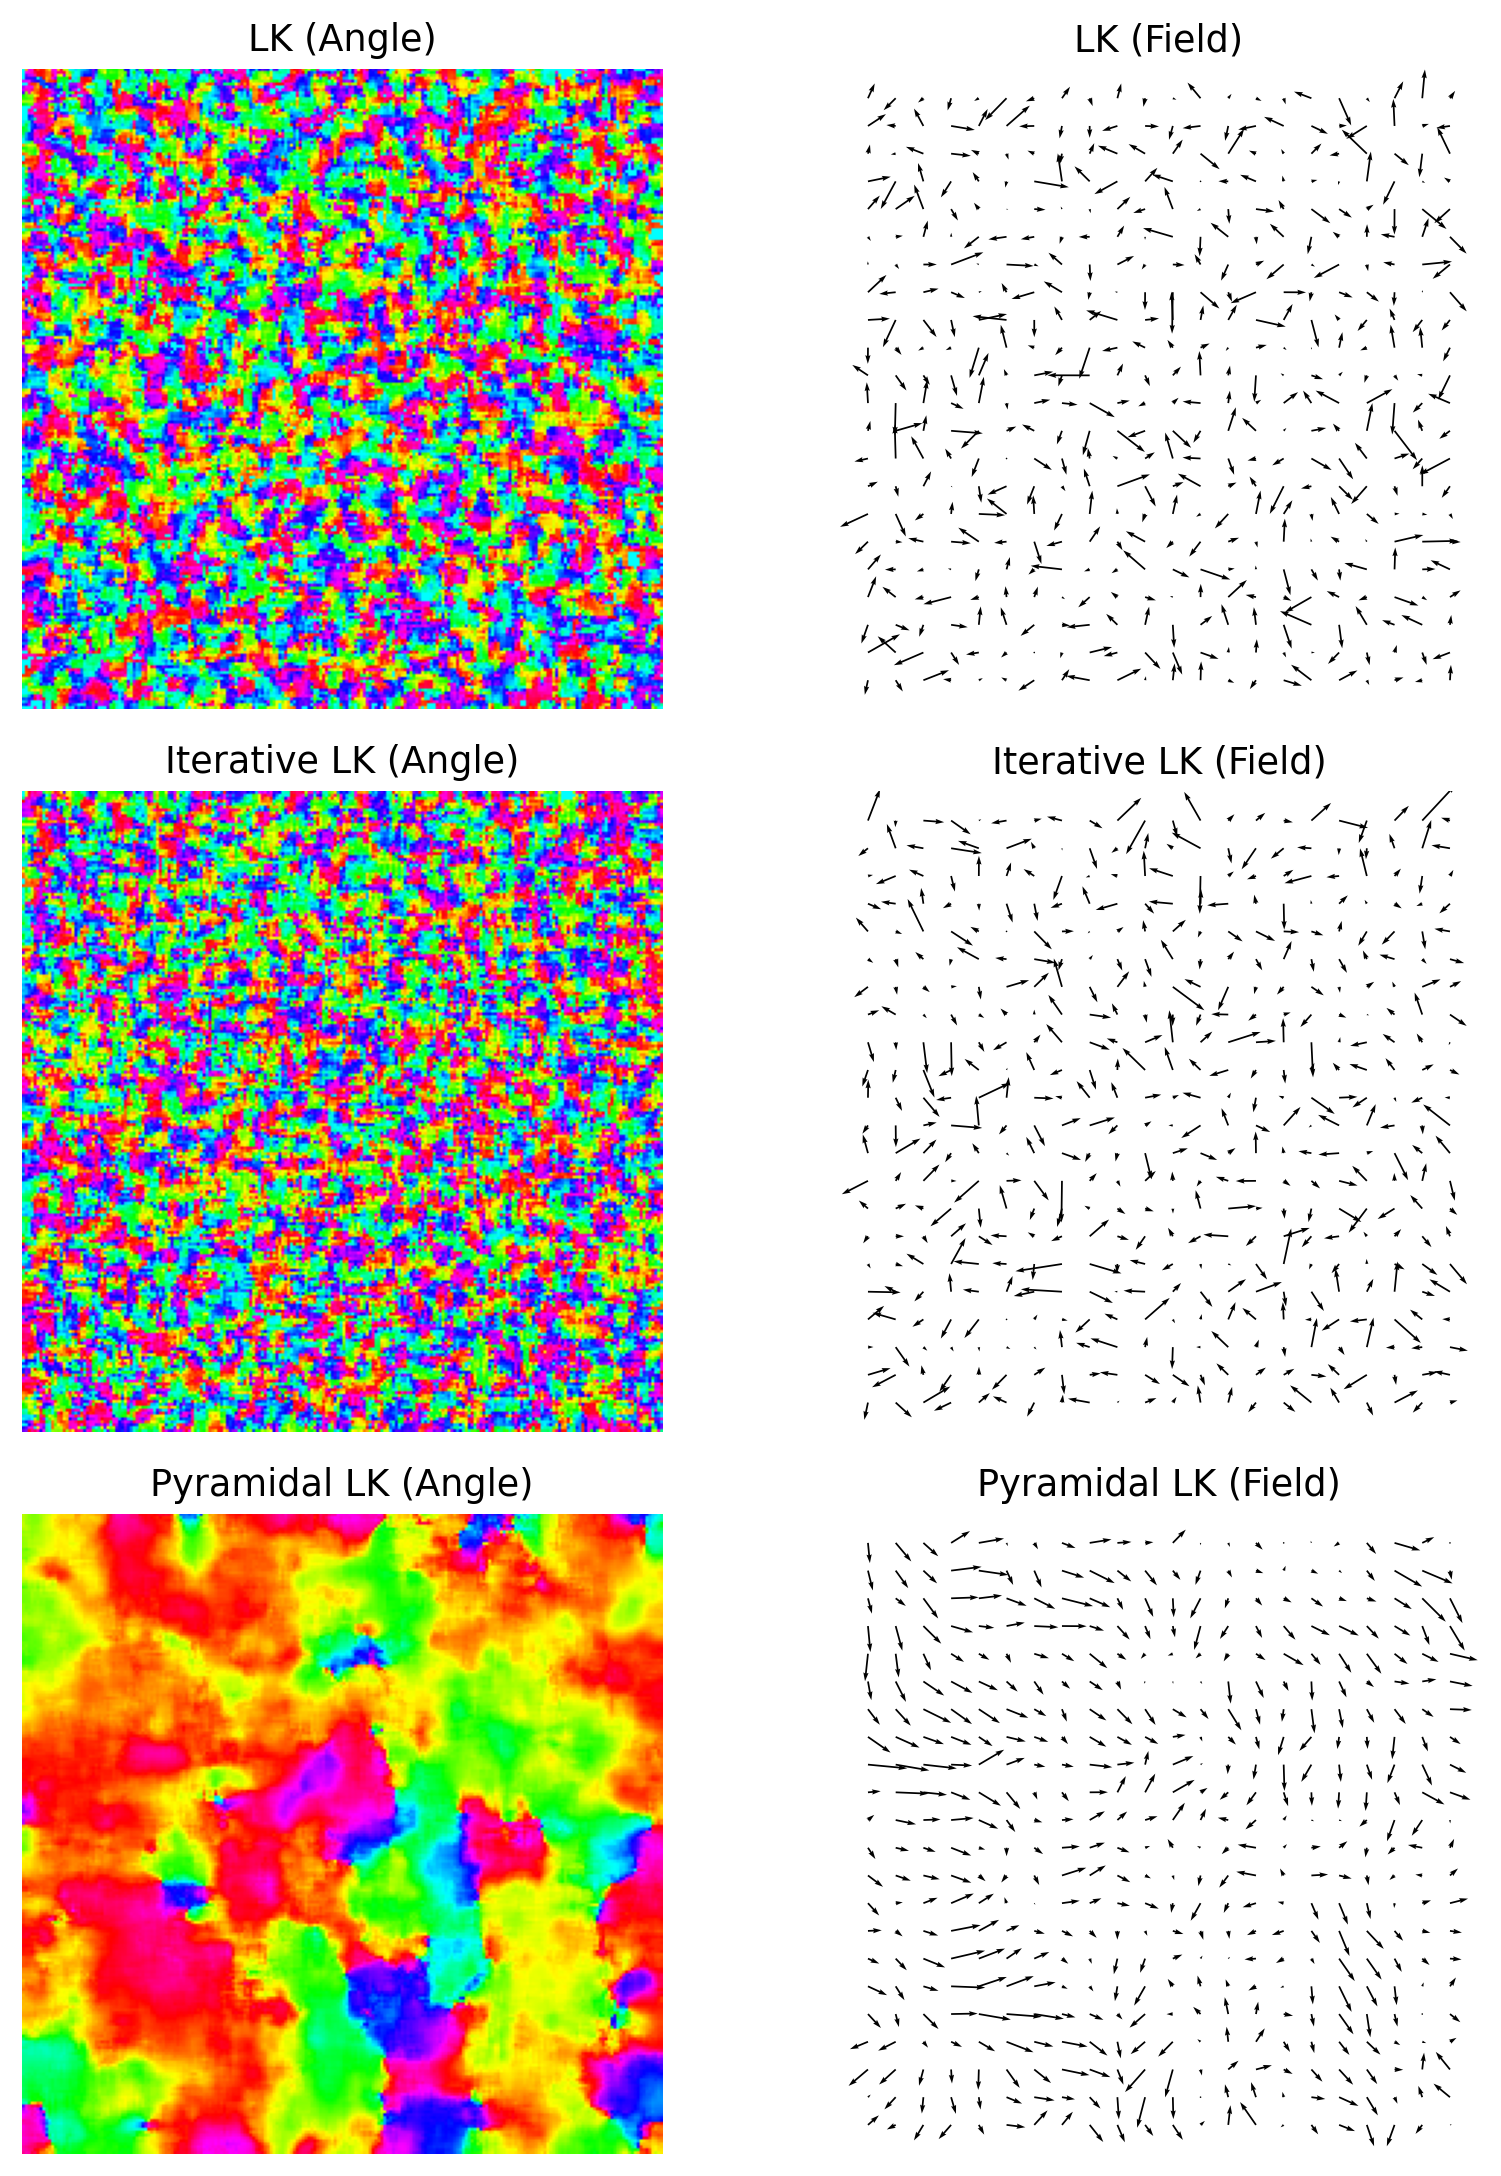
\includegraphics[width=1\columnwidth]{figure_pyr_flows.png}
    \caption{Additional part: LK (row 1), iterative LK (row 2), pyramidal LK (row 3).}
    \label{fig:pyr_flows}
\end{figure}

\section{Conclusion}
I implemented both required methods and tested them on synthetic and real data.  
HS gave denser flow and lower residual. LK ran much faster.  
On real images, LK stayed sensitive in low-texture regions.  
LK-based HS initialization reduced runtime a lot with a small quality drop.  
I also implemented pyramidal LK, but this part still needs parameter tuning.

\end{document}
